\section{MPI quick tuning}


\chapterDescription
  {
    Around 15 minutes.
  }
  {
    A working MPI code.
  }


This section collects a couple of really primitive measurements to make your
code faster.

\subsection{Filter out log statements}

It is probably to simple to mention, but all our teams from time to time forget
this. 
One of the major things slowing down codes is writing to the terminal. 
So adding a few additional log filters can significantly speed up your code.



\subsection{Switch off load balancing}

Most of Peano's load balancing algorithms (at least the ones coming along with
the standard package) rely on a central node pool.
If a rank decides that it would be advantageous to split up its domain, it sends
a request to the first rank whether there are any idle nodes available.
If your code already uses all ranks, this is a time consuming process that
suffers from latency.
If you know a prior that the load balancing is static and no further splits of
subdomains are possible, it does make sense to switch the load balancing off.
There is a routine \texttt{activateLoadBalancing} operation on the load
balancing oracle to do so.

This operation has to be called on each individual rank, i.e.~you can switch 
the load balancing on and off on a rank-per-rank basis. There are basically two
variants/patterns to disable the load balancing:
\begin{enumerate}
  \item You may introduce a new mapping that does nothing besides switching the
  load balancing off (typically in \texttt{beginIteration}). You then merge this
  mapping into your other adapters.
  \item You add a new bool to your state. In the global runner you set this
  boolean flag once you want to switch the load balancing off. The state then is
  successively propagated to the workers. In \texttt{beginIteration}, you
  analyse this bool (in any mapping) and you switch off the load balancing if
  the flag is set.
\end{enumerate}

Peano also offers the opportunity to invoke a
global step on all ranks prior to an \texttt{iterate} call.
This feature can be used to switch off the load balancing, too:

\begin{code}
void picard::runners::Runner::runGlobalStep() {
  peano::parallel::loadbalancing::Oracle::getInstance().activateLoadBalancing(false);
}


int picard::runners::Runner::runAsMaster(...) {
  ...
  
  repository.runGlobalStep(); // on all other ranks
  runGlobalStep();            // and locally, too
}
\end{code}

\noindent
As clarified in the documentation of the operations (see the autogenerated
header files of your repository, e.g.), you have to be careful if you follow
this variant:
You are never allowed to run a global step if any rank is involved in a join or
fork. 


\subsection{Reduce data exchange with global master}

\begin{smell}
  It seems that rank 0 is involved in lots of data exchange (the performance
  analysis says that it is a neighbour data exchange bottleneck), and we see
  that rank 0 holds a significant number of total vertices and cells.
\end{smell}

Peano takes the computational Domain (the unit square, e.g.) and embeds it into
a $3^d$ patch. This surrounding patch is held by rank 0 being the global master.
This rank deploys the central element, i.e. the whole domain, immediately to
rank 1 and sticks himself with administrative duties (the node pool server
realising domain decomposition decisions, e.g.) only. 
We have a situation as sketched below on the left:

\begin{center}
  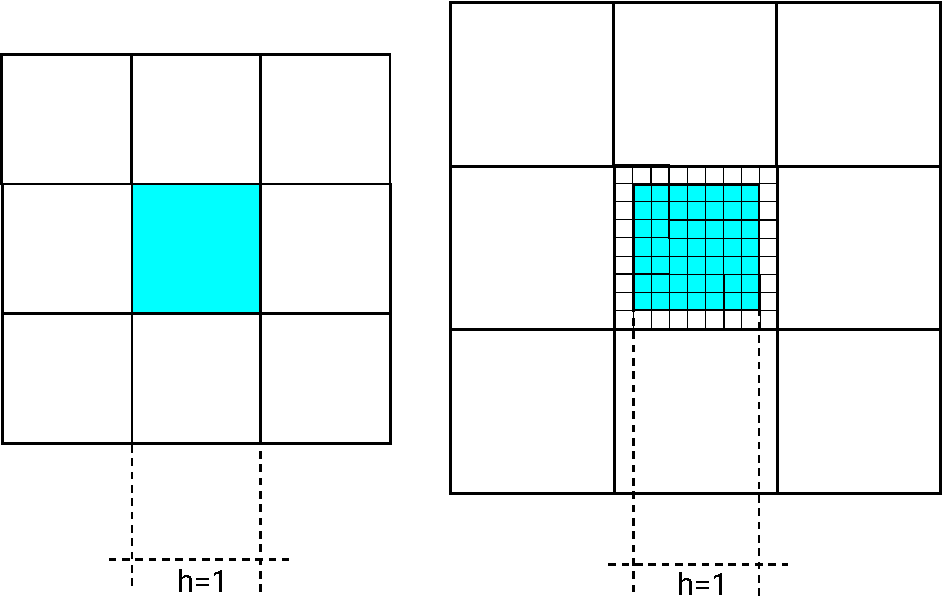
\includegraphics[width=0.5\textwidth]{62_quick-tuning/domain-layout.pdf}
\end{center}

The global master 0 deploys the real domain (filled) to rank 1 and then rank 1
continues to split up its domain further.
Though rank 0 has deployed all cells to other ranks, still many workers of rank
1 (up to eight) are adjacent to rank 0. 
If they refine (and they most probably will do as most PDE solvers refine along
the domain boundary), there is a pretty huge refined surface that connects each
of the eight workers of rank 1 with rank 0. 
And now rank 0 becomes a bottleneck though rank 0 does no computation at all.

\begin{center}
  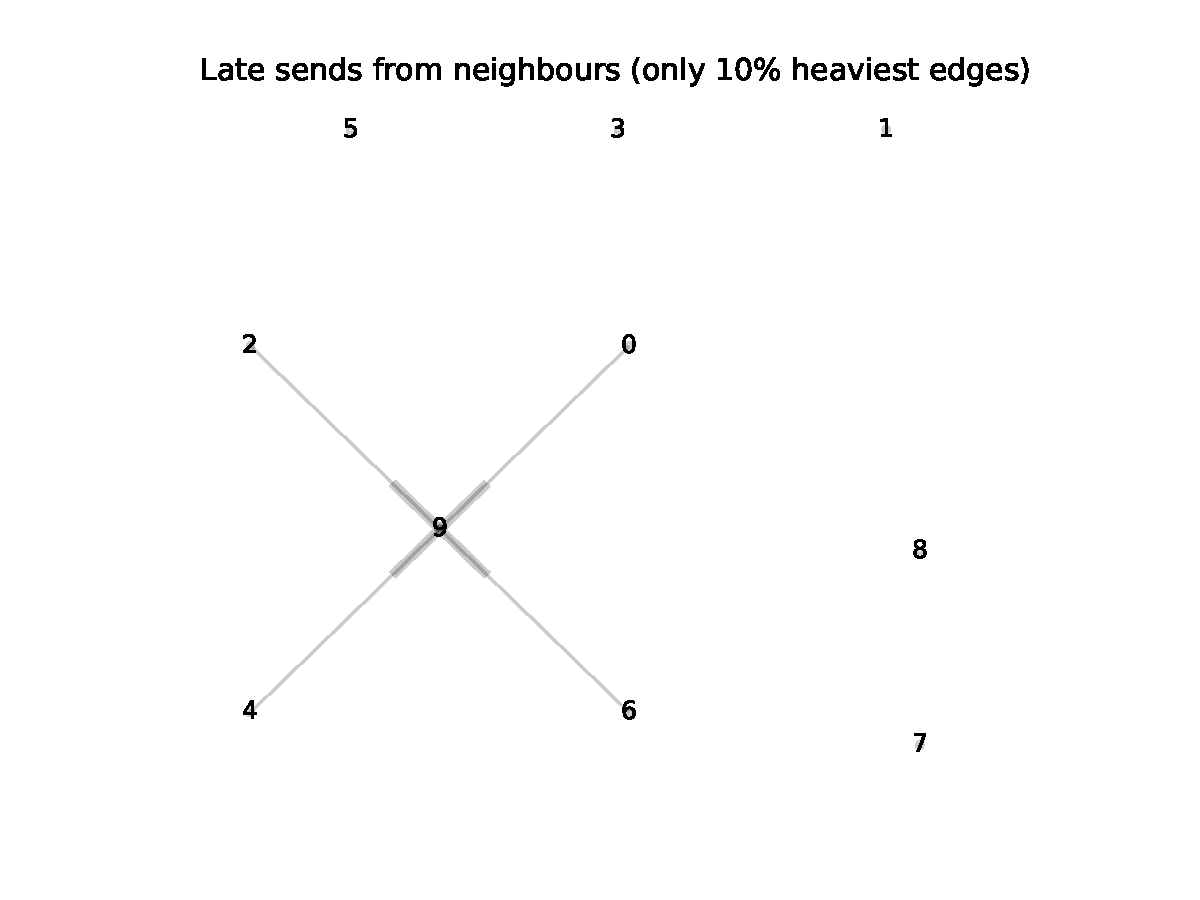
\includegraphics[width=0.45\textwidth]{62_quick-tuning/boundary-data-exchange.pdf}
  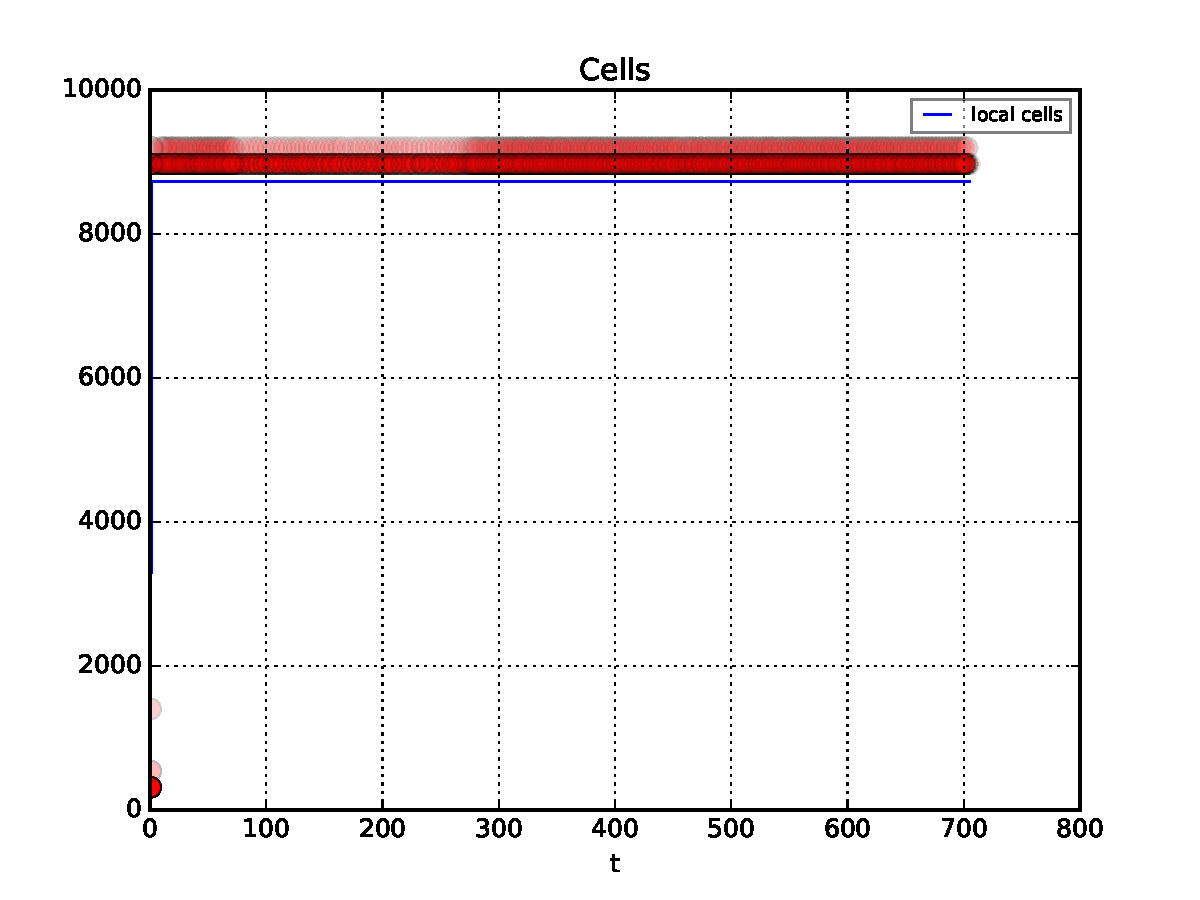
\includegraphics[width=0.45\textwidth]{62_quick-tuning/local-cells-rank-0.pdf}
  \\
\end{center}
  {
  \footnotesize
  Smells on the global master in the performance analysis output.
  Standard run on unit square, regular grid, $d=2$ with 10 ranks. 
  Left: Rank 0 is a boundary data exchange bottleneck though it has deployed all
  of its work to rank 1.
  Right:
  Rank 0 holds a significant number of cells (solid line) cmp.~to the cells on
  the other ranks (red dots) though it has deployed the domain completely.
  \vspace{0.8cm}
  
  }

One solution is to extend the bounding box around the computational domain by a
halo region.
For a unit square, using an offset of $-1/7 \times -1/7$ and a bounding box
size of $9/7 \times  9/7$ has proven of value. 
This way, all halo cells of rank 0 are sufficiently away from the domain's real
boundary. 
So, if a worker of rank 1 refines, it does not share additional Vertices with rank 0. 0 is not a bottleneck anymore.
The drawback of this approach is that the first few coarser levels on the ranks
are not involved in any computation (makes a difference for multigrid, e.g.) as
they overlap the whole computational domain. 
Only the third or fourth level of the spacetree actually holds valid compute
data.

To identify whether you can benefit from this technique, try a simple run with a
regular grid and only two ranks. 
In this case, you should not see any speedup, as all work is deployed by rank 0 to rank 1. 
However, you should also not observe a significant runtime penalty. 
If you do observe a penalty, try to realise this fix:


\begin{code}
// the actual computational domain remains the same - we are not altering the
// physics
peano::geometry::Hexahedron geometry(
  tarch::la::Vector<DIMENSIONS,double>(1.0),
  tarch::la::Vector<DIMENSIONS,double>(0.0) );
myproject::repositories::Repository* repository = 
  myproject::repositories::RepositoryFactory::getInstance().createWithSTDStackImplementation(
  geometry,
  tarch::la::Vector<DIMENSIONS,double>(9.0/7.0),   // has been 1.0 before
  tarch::la::Vector<DIMENSIONS,double>(-1.0/7.0)   // has been 0.0 before
  computationalDomainOffset );
\end{code}

\begin{remark}
If you use non-cubic domains, you have to scale both quantities with the size of
the domain's bounding box.
If you know a prior how many regular levels your grid will have, then you should
choose the bounding box such that one cell of the finest grid overlaps into the
outer region. 
In the example above, the minimal level would be two.
If you use a tailored/sophisticated load balancing oracle, this oracle should be
aware of this level as well.
\end{remark}



\subsection{Work with better balanced domains}

\noindent
Peano controls its load balancing via MPI oracles and a node pool strategy. 
On the long term, there is almost no way around tailored MPI domain
decomposition routines.
There is however a mpi balancing toolbox that provides some generic load
balancing routines that are superior to the default implementations in the
kernel.
So it can be wise to try out these (and perhaps use them as starting point for
better load balancing).

\begin{smell}
  The load balancing yields a strongly irregular load decomposition though the
  problem is very regular and geometrically simple.
\end{smell}

\noindent
With the help of the performance analysis such a behaviour materialises in
ill-balanced logical topology graphs.
The visualisation should, for a regular domain and a regular grid, yield a
tree-type graph where most ranks with the same distance from the root node 0
have roughly the same number of children.

\begin{center} 
  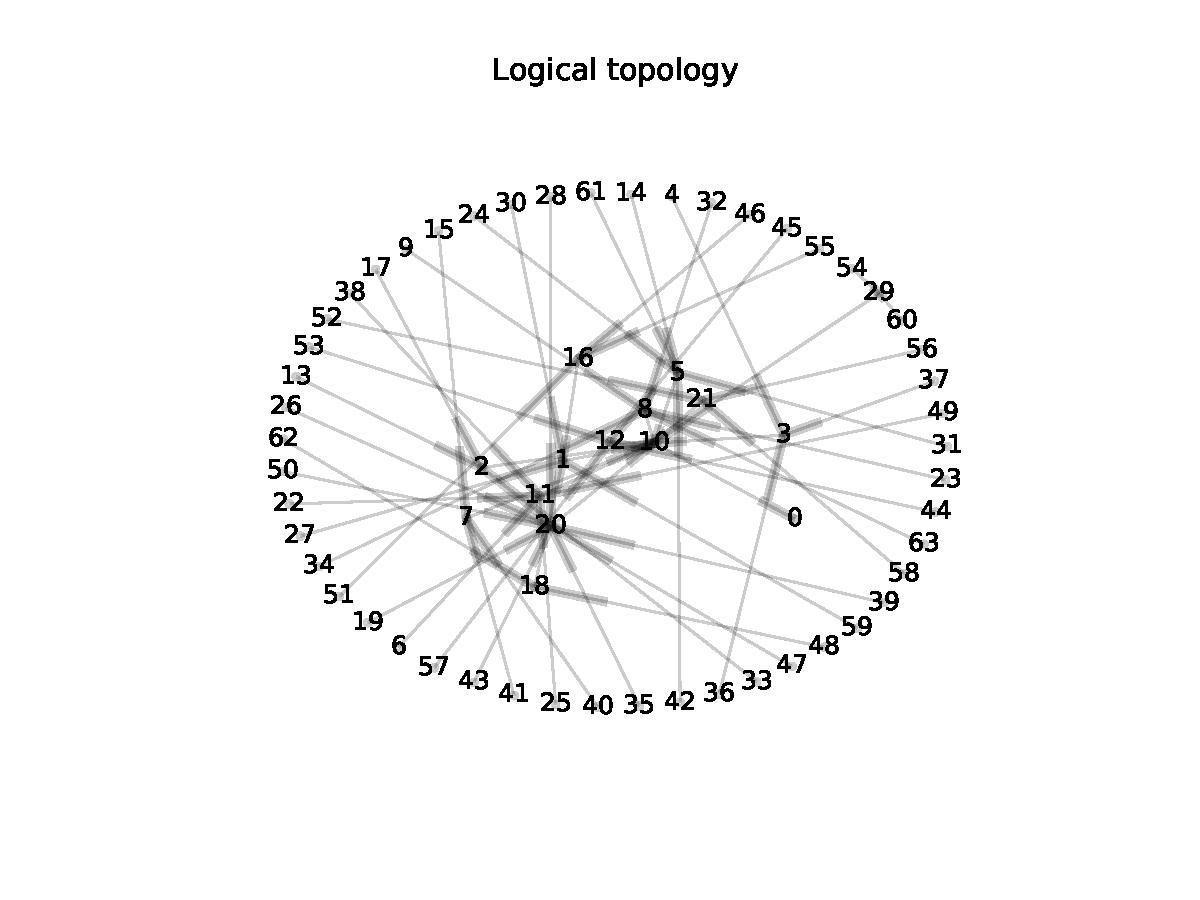
\includegraphics[width=0.4\textwidth]{62_quick-tuning/topology.pdf}
  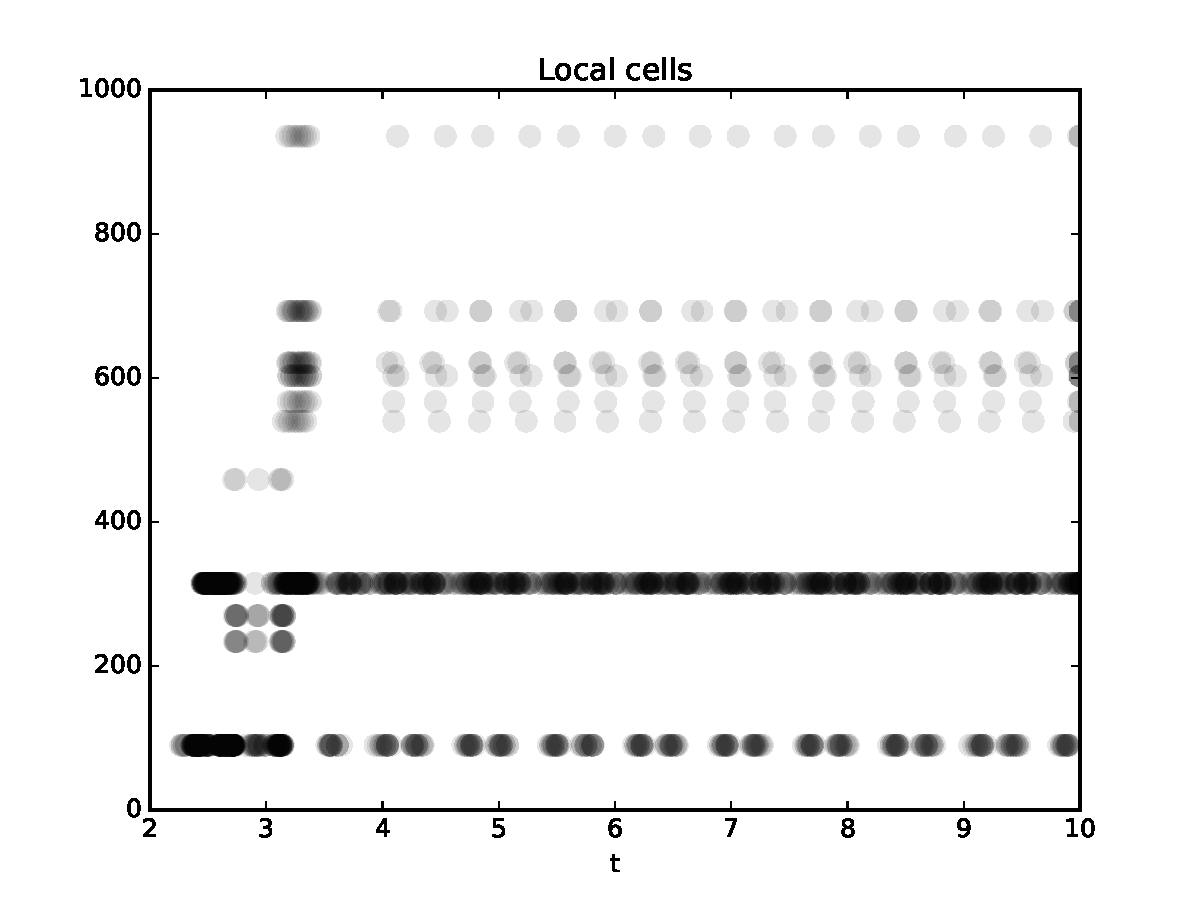
\includegraphics[width=0.4\textwidth]{62_quick-tuning/local-cells.pdf}
\end{center}

\noindent
Another smell indicator is a fork table where too many levels are actually
populated. 
If you have a regular grid on the unit square---you might already use a slightly
modified bounding box; in this case you have to adopt the esimates---1 nodes
should be used on level 1, 8 nodes should be used on level 2, $8 \cdot 8$ nodes
should be used on level 3, and so forth.
If level 4 and 5 for example are used while level 3 comes along with smaller
fork counts, it might be that one rank in the domain forks aggressively and
leaves no idle ranks for the other ranks working on other subpartitions.

A third indicator for such a behaviour is the overview over the local cells.
All local cell counts should roughly be in the same order of magnitude. 
At least there should not be many groups of ranks with different cell counts.
In the picture above, this does not hold.
It implies that we have ill-balanced partitions.

To solve the problem, you can use one of the \texttt{Balancing} classes from the
toolbox \texttt{mpibalancing} in your \texttt{runAsMaster} routine.
Please consult their header for detailed information on the class behaviour.
Most balancing strategies require you to invest some work to feed the
oracles a cost model.



\subsection{Increase the grid regularity}

If grid parts change or are strongly adaptive, Peano does not decompose these
grid regions through MPI. 
Furthermore, most load balancing strategies can quickly decompose regular grid
levels, while decomposing adaptive regions is tricky.

\begin{center}
  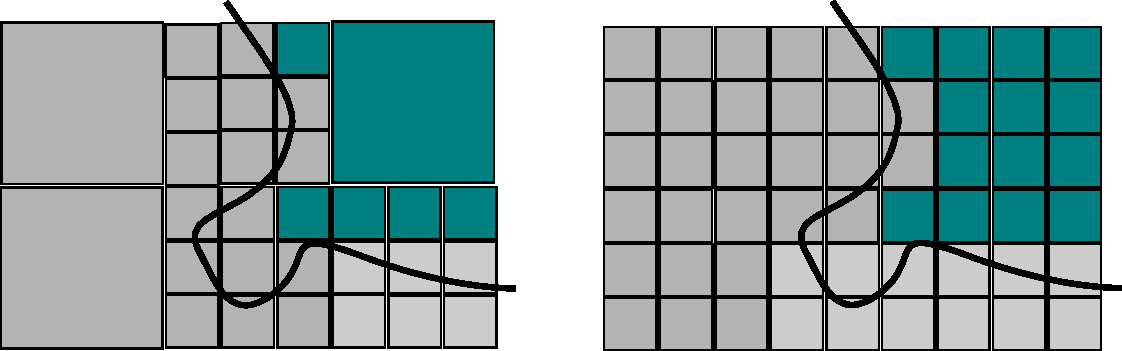
\includegraphics[width=0.6\textwidth]{62_quick-tuning/regularity.pdf}
\end{center}

\noindent
In the example above, Peano often struggles to split up the boundary as the
adaptivity pattern around the boundary is complex.
We often end up with a situation where the whole boundary ends up on one rank.
If we increase the grid regularity manually (right example), the scaling
improves.

\begin{smell}
  The domain decomposition works properly. Nevertheless, some ranks responsible
  for the boundary are slow (w.r.t.~boundary data exchange) though they are
  properly balanced.
\end{smell}

\noindent
To increase the regularity, you can manually tailor your adaptivity criterion or
you can increase the value returned by the oracles.
They prescribe a maximum regularity level that is also anticipated outside of
the domain and thus avoids adaptive grids outside of $\Omega $ up to a certain
level.

\subsection{Avoid races for idle ranks}

\begin{smell}
  The balancing seems to work fine for small rank counts (up to 256 ranks,
  e.g.). If I use more ranks, the balancing at first glance seems to be fine,
  but some ranks just seem to be more successful in booking additional ranks.
\end{smell}

\noindent
This smell manifests quickly if you use the script
\texttt{domain-decomposition-analysis.py} from Peano's
\texttt{performanceanalysis} directory. 
We discuss this at hands of the graphs below running a job with 512 ranks: 

\begin{center}
  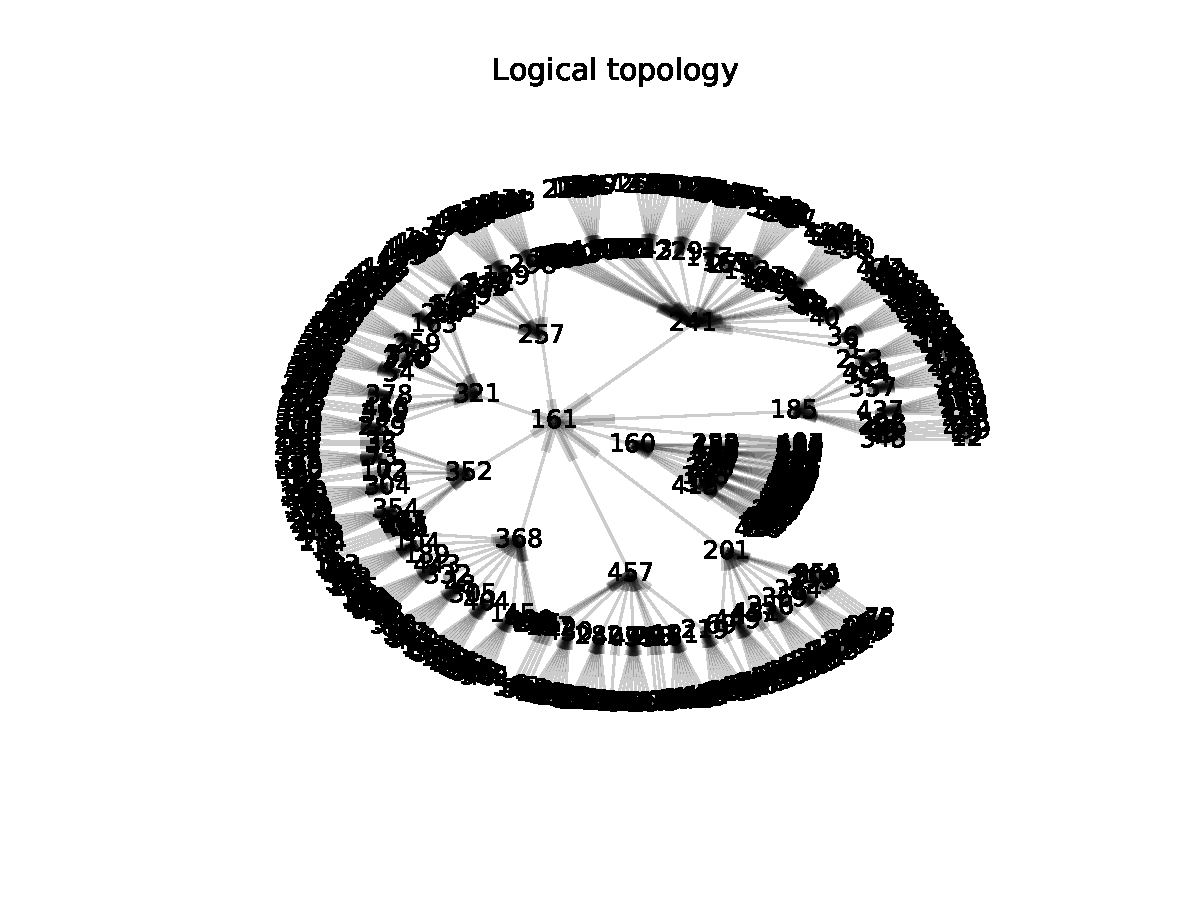
\includegraphics[width=0.3\textwidth]{62_quick-tuning/rank-races.pdf}
  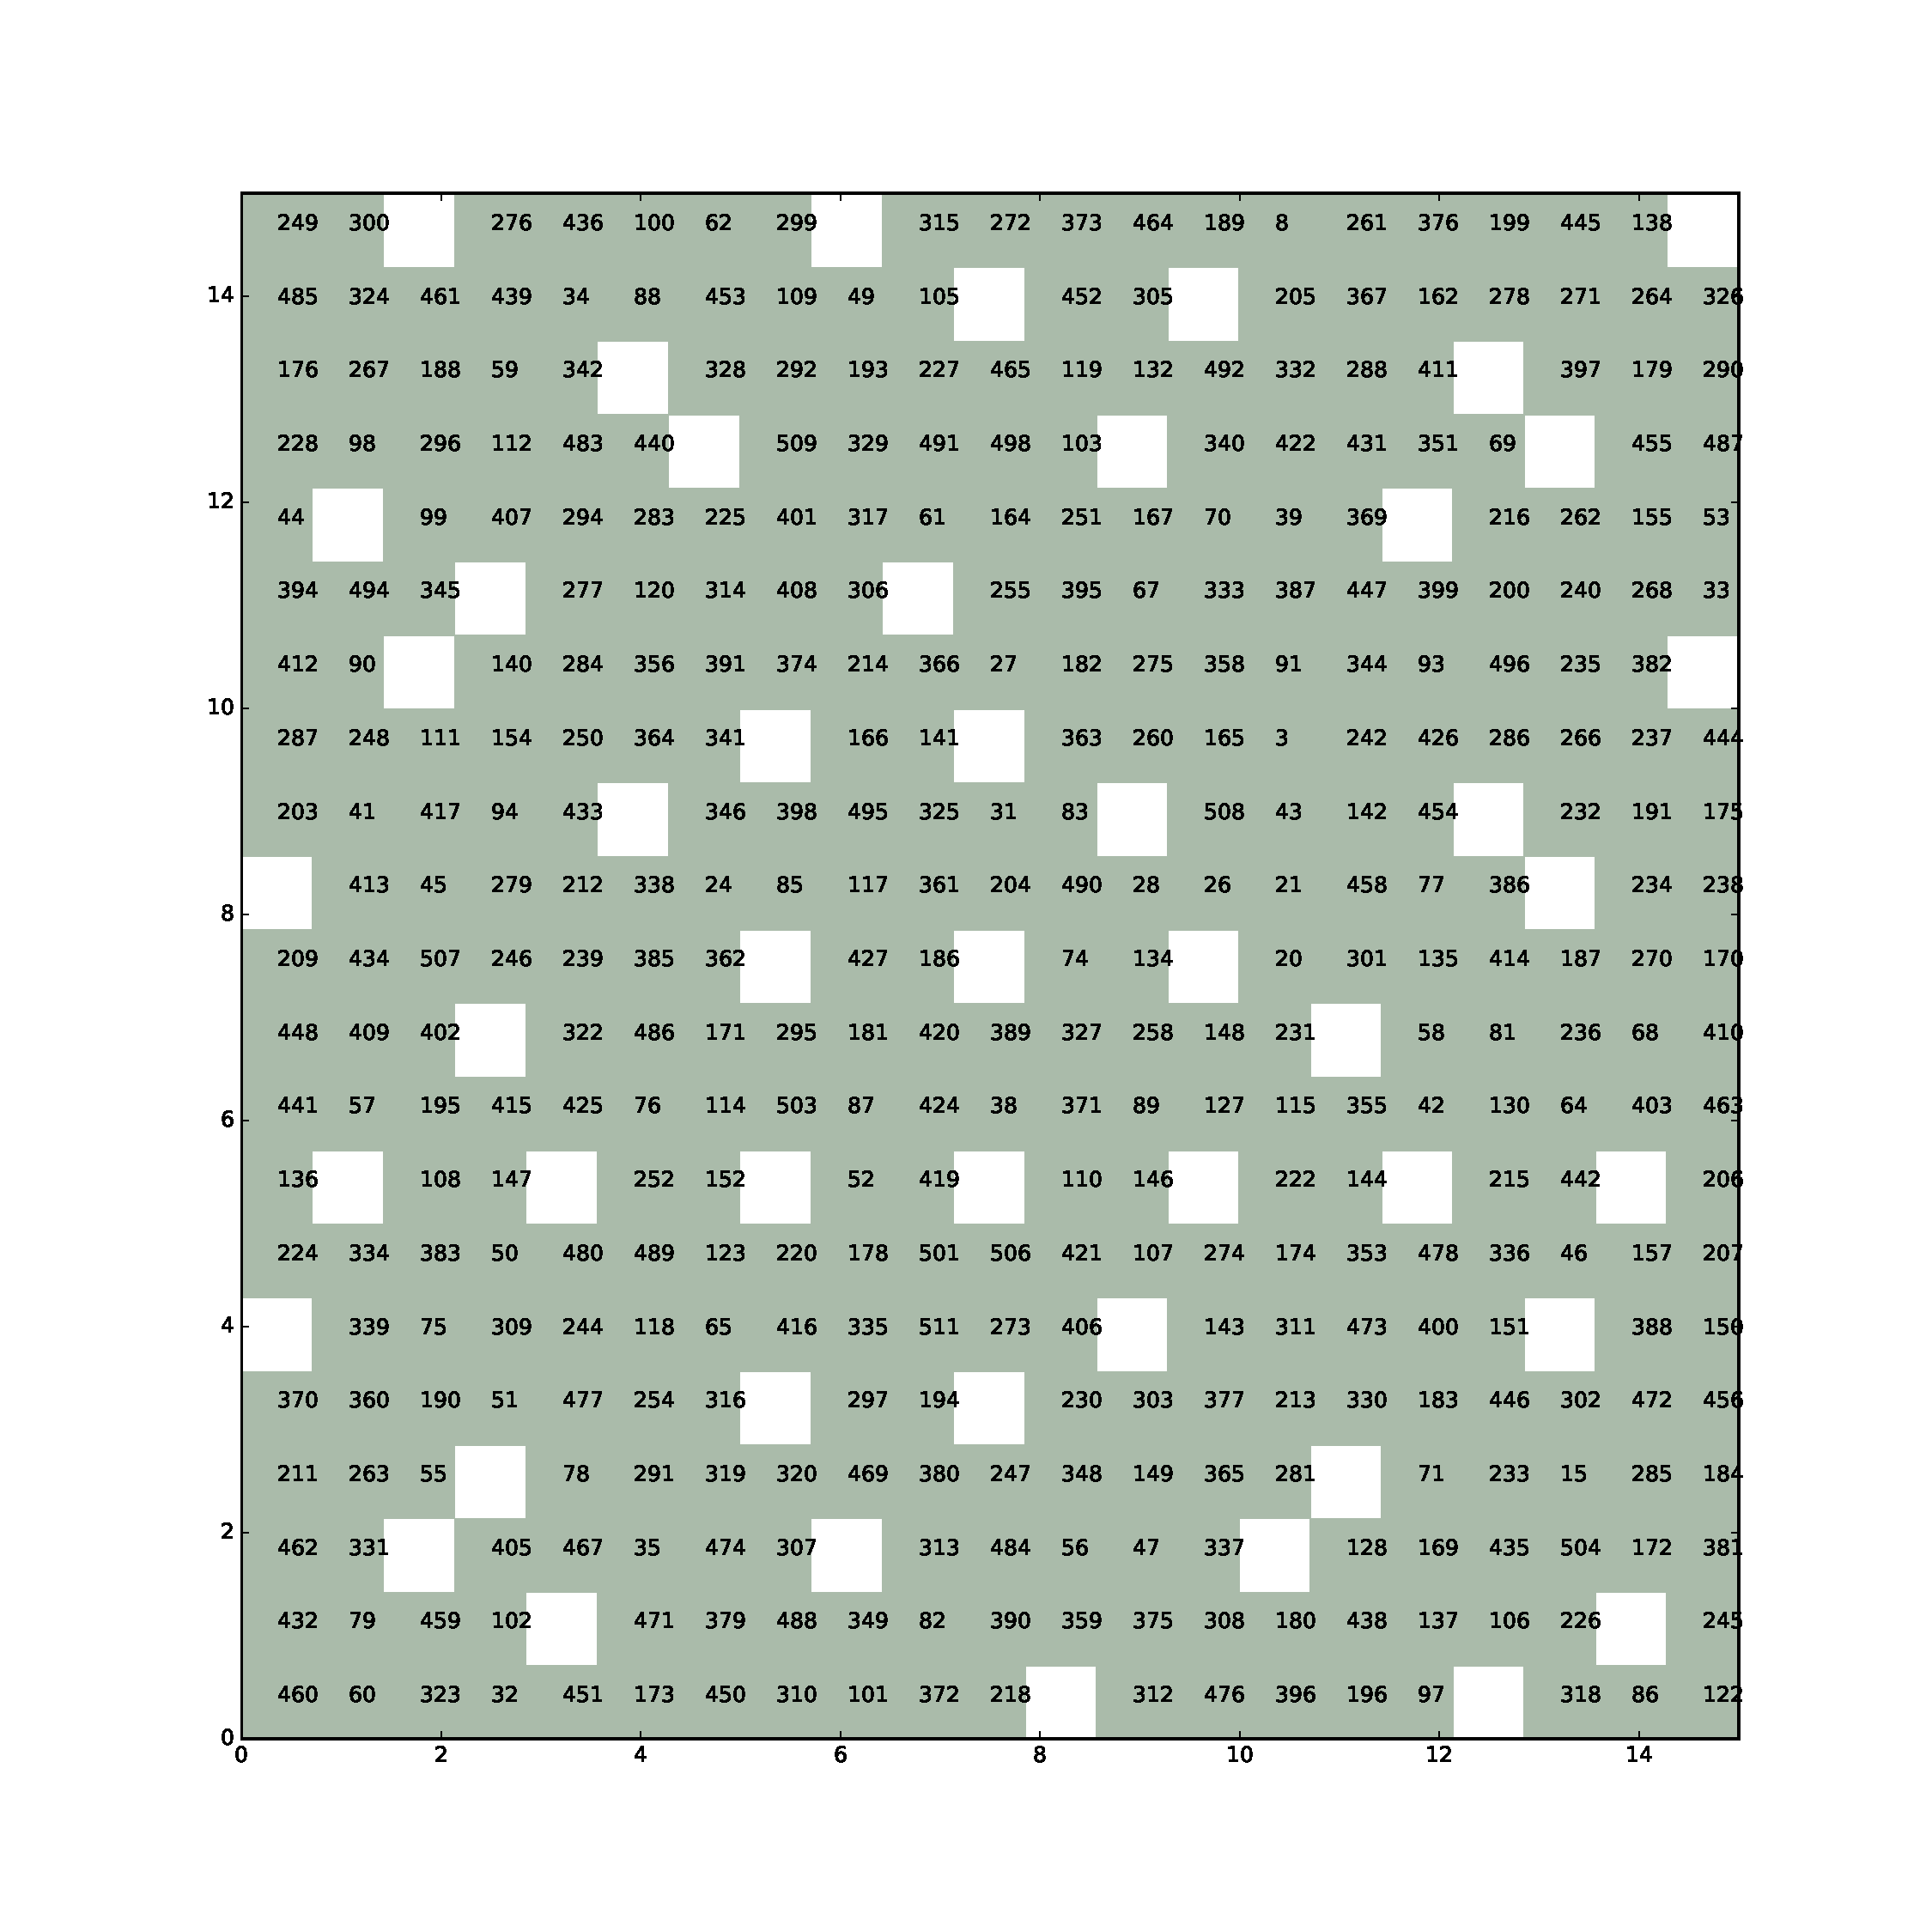
\includegraphics[width=0.3\textwidth]{62_quick-tuning/rank-races-level4.pdf}
  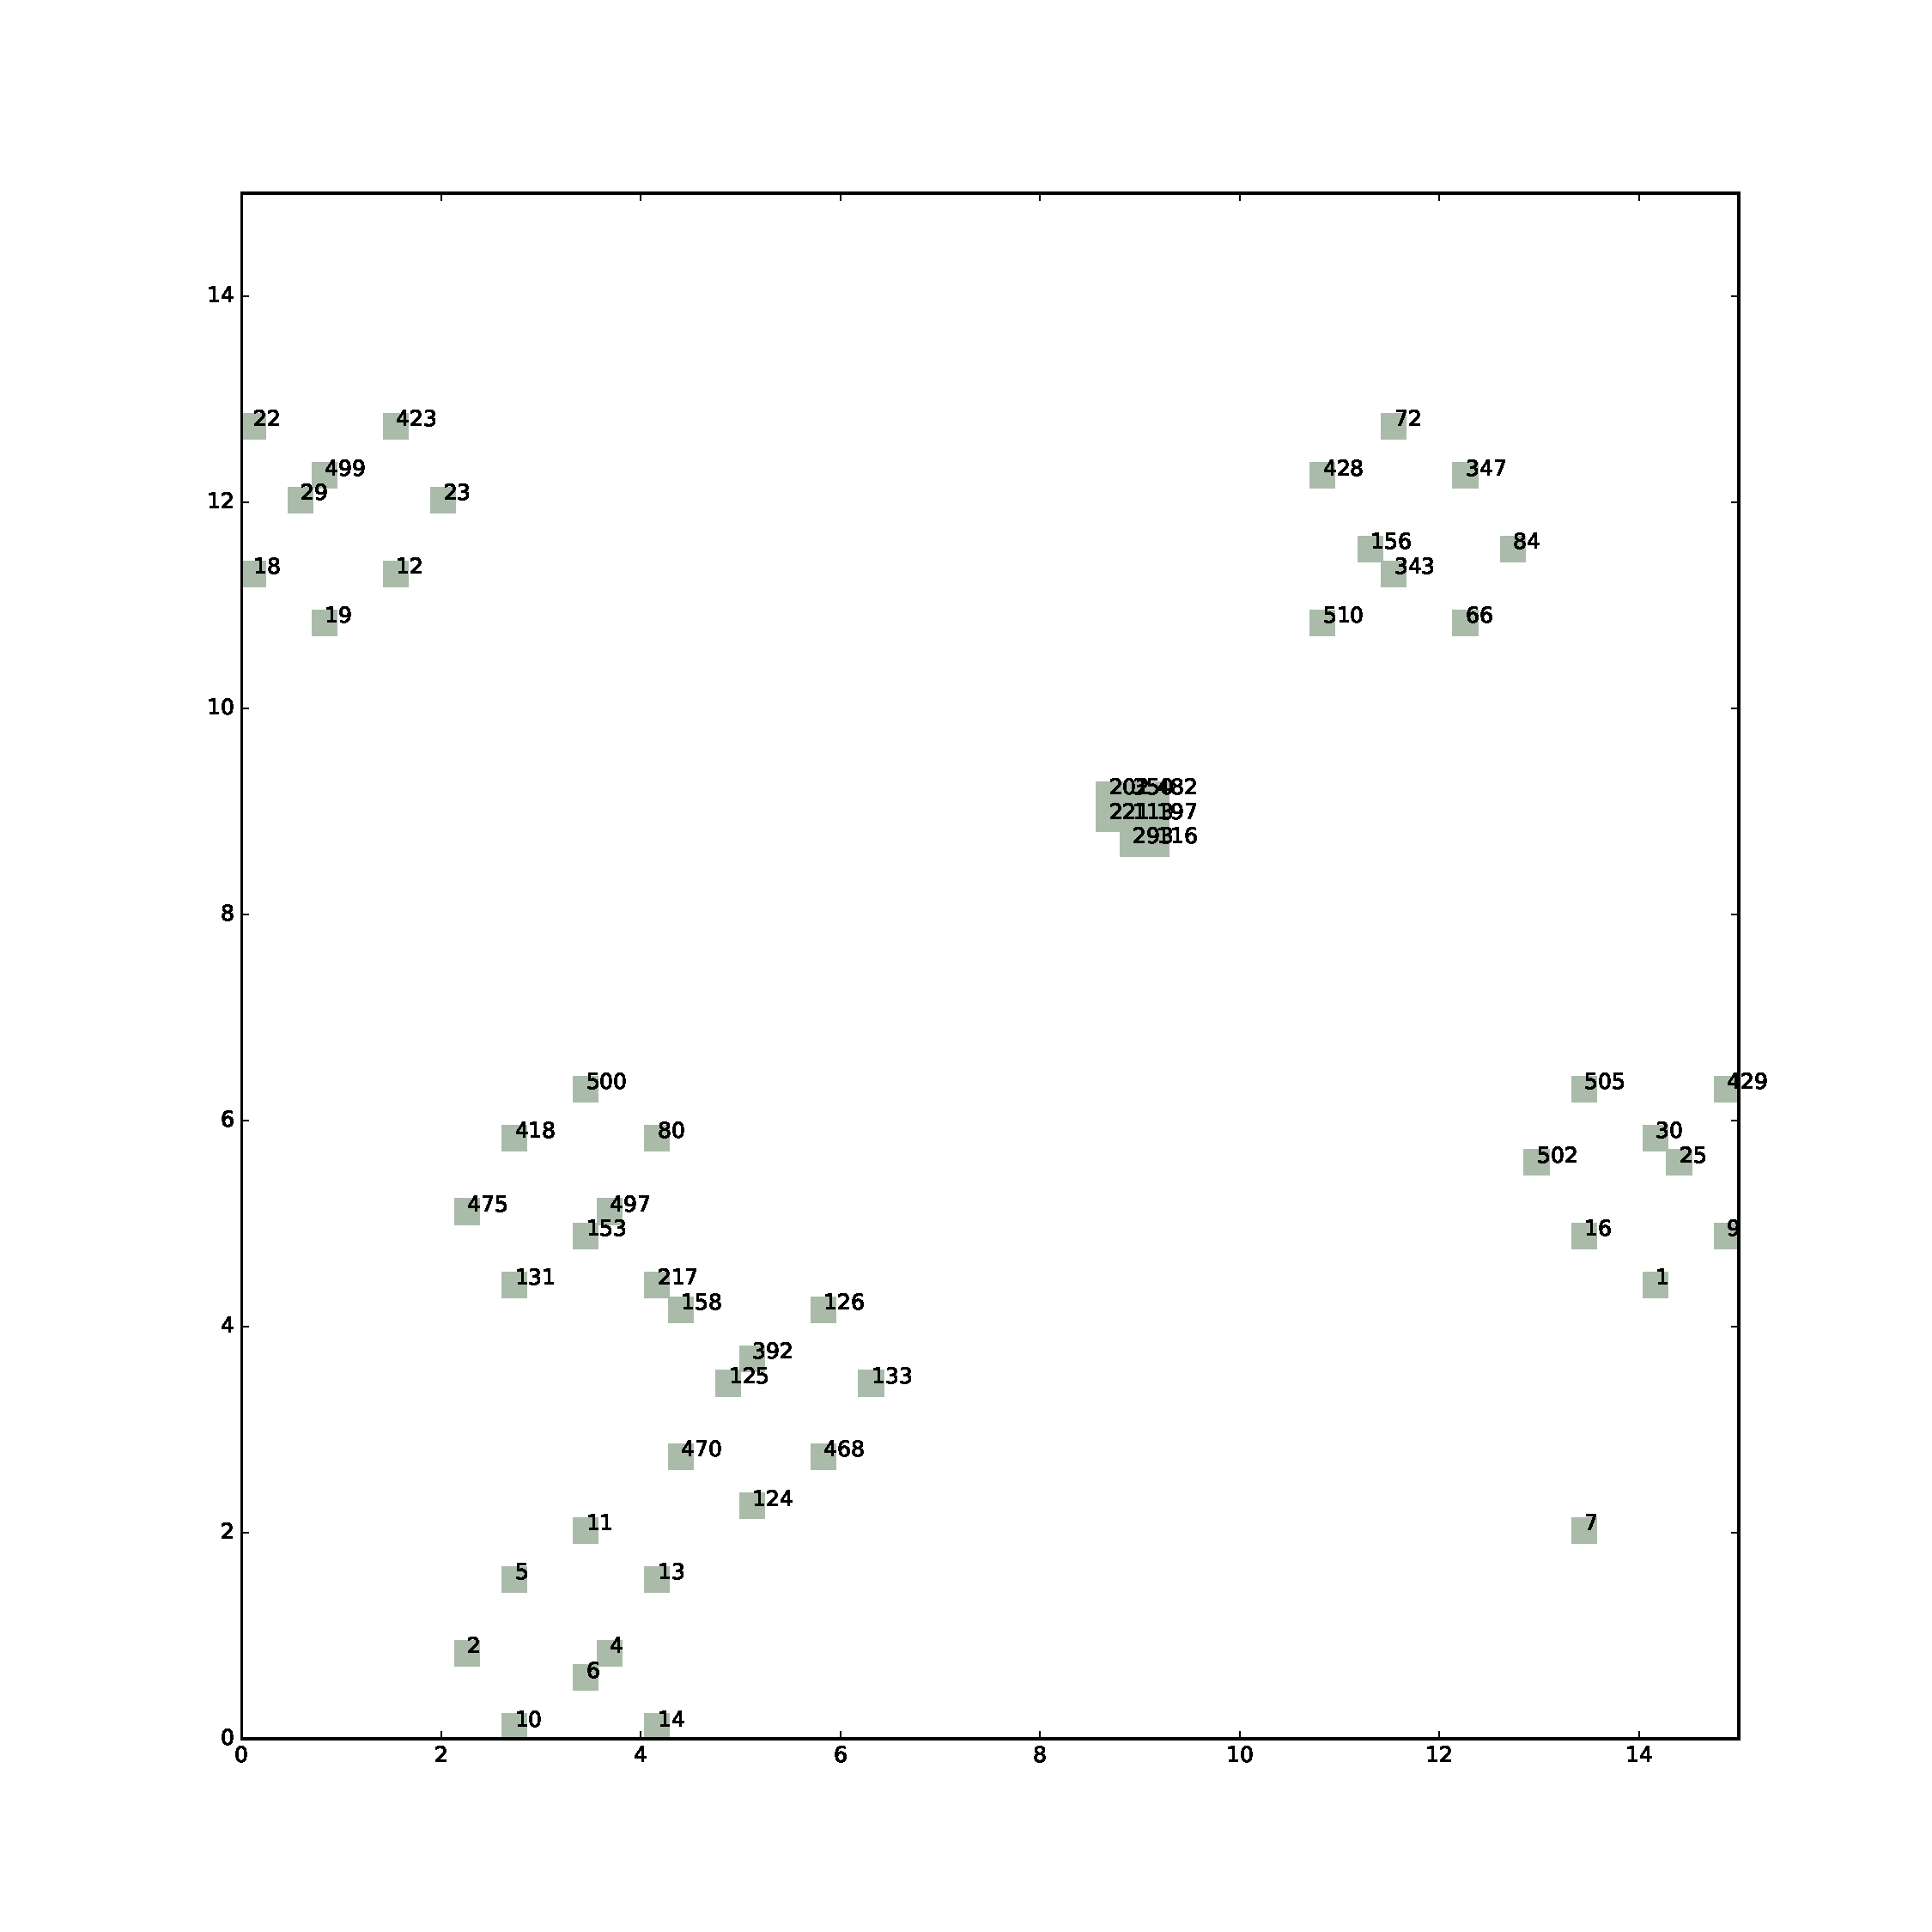
\includegraphics[width=0.3\textwidth]{62_quick-tuning/rank-races-level5.pdf}
\end{center}

\noindent
The balancing seems to be reasonable (left graph), and the work per rank
graph (not shown here) shows a reaonsable work distribution.
We continue to study the first four levels of the multiscale grid 
and still all results seem to be very reasonable. 
Level one to three are not shown, the middle graph above is level four.
Each rank (we are tackling a $d=2$-dimensional setup) forks per level eight
cubes to other rank.
On level four (right) and five (not shown) however, we see a very localised rank
employment.
This means that some ranks responsible for level three are very successful in
booking additional ranks for their subdomains, while others are left
empty-handed.

The best fix to this problem is to write a node pool strategy that is aware
which rank should be used for which subdomain and how many additional
worker ranks any rank is allowed to book.
This is a laborious endeavour (though required for extreme-scale runs). 
For the time being, Peano offers a fair node pool strategy where the node pool
gathers rank requests and then hands out ranks to those ranks first that haven't
got any additional ranks yet.
This strategy is only to be set on the global master.

\begin{code}
tarch::parallel::NodePool::getInstance().setStrategy(
  new mpibalancing::FairNodePoolStrategy()
);
\end{code}

\noindent
It allows you furthermore to instruct the balancing now many MPI ranks are
placed on each individual node. 
The strategy then tries to assign each node roughly the same number of ranks for
any level.
For regular grids, this helps to keep the peak memory requirements per node
bounded.


\subsection{Next \ldots}




@todo hier auch was rein zu machine-specific lb -> Das gehoert aber nicht hier
rein, sondern ist schon sophisticated (also nimmer quick)

GLeiches gilt fuer den Rest

@todo Die drei regular grid specs (maximal mesh width, overlap of DD und oracle)
muessen synchronisiert sein.

@todo dann neues Time stepping und eliminieren von Reduktionen

